\chapter{Partial Charge Analysis}
\label{ch:part_char}

Having optimized structures and a quantitative point of comparison (namely, the potential maps), the last piece needed to parameterize a force field is the partial charges on the constituent water molecule atoms. 

Many different methods exist for assigning partial charges to atoms, and a systematic process for deciding which is best for the system at hand is desired. Since it is not known \textit{a priori} what the partial charge distribution should look like for the extra-framework water molecules, known systems are used to benchmark the partial charge analysis techniques under the 
DFT assumptions made thus far. Specifically, the total dipole for the monomer, dimer, and trimer water cases are calculated and compared to literature. 

Once a suitable technique is selected, a similar investigative technique as used in the structural optimization and potential map calculations is employed. That is, partial charge analysis is performed on the vacuum-geometry and beryl-geometry water molecule arrays in vacuum followed by analysis on the framework-inclusive system. 

    \section{Benchmark}
    \label{sec:benchmark}
    
    \paragraph{Overview} As mentioned above, there exists different partial charge analysis techniques, each with their own advantages and disadvantages. Specifically, four different techniques are compared: (1) Bader Charge Analysis [\textbf{CITATION}], (2) DDEC analysis with ChargeMol [\textbf{CITATION}], (3) DDEC6 analysis [\textbf{CITATION}], and (4) centers of Maximally Localized Wannier Functions (MLWF) [\textbf{CITATION}]. 
    
    For each method, the total dipole for the monomer, dimer, and trimer (MDT) water systems is calculated on a structure optimized under the same assumptions (basis set, functionals, etc.) as used in the rest of the work. For methods 1-3, results were qualitatively in agreement with literature values but varied by up to a factor of two otherwise. It is the latter method, using the centers of MLWF, that proved the most accurate; however, issues of convergence appeared that will be discussed below.
    
    \paragraph{Procedure} As discussed briefly in Section \textbf{THEORY SECTION NUMBER}, determining the partial charge via the MLWF is conceptually trivial. In short, a basis transformation from the Bloch functions to non-unique Wannier functions is performed, and then the spread of said Wannier function is minimized to obtain the unique MLWF. From the MLWF, the center can easily be calculated, and this center can be viewed as the classical location for the negative charge. (See theory section or [\textbf{MLWF review citation}] for a more in-depth explanation.) 
    
    Fortunately, it is possible to compile VASP with the VASP2WANNIER library and use said library as a post-processing step on the self-consistent calculations performed for the potential map analysis. This post-processing produces an input file for the Wannier90 software package [\textbf{citation}], which calculates the actual Wannier centers. In general, the number of centers is equal to the number of electrons in the system, but since all calculations performed here are not spin-polarized, the number of centers is equal to \textit{half} the number of total electrons. Additionally, pseudopotentials are used in lieu of including core electrons. This results in 8 electrons---and therefore, 4 wannier centers---per water molecule.
    
    Once calculated, the Wannier centers need to be assigned to the proper water molecule. This is accomplished with a simple Python script that utilized the ASE library to find the two closest oxygen atoms and four closest Wannier centers (including periodic images) for each oxygen atom. Each set of oxygen atom, two hydrogen atoms, and four Wannier centers constitutes a water molecule. Using the position and charge ($+6e, +1e, +1e, -2e, -2e, -2e, -2e$ respectively, for elementary charge $e$) for each element, the molecular and total system dipole can be calculated using the classical, discrete definition
    
    \begin{equation}
    \label{eq:dipole_def}
        \Vec{p} = \sum\limits_{i=1}^{N} q_i \Vec{r}_i,
    \end{equation}
    
    \noindent for sum over $N$ total elements, with charge $q_i$ and position $\Vec{r}_i$ of element $i$. Note, it is actually the magnitude of the total system dipole moment $ p = |\Vec{p}|$ that is of particular interest and will be compared to literature values for this benchmark.
    
        \subsection{Convergence Issue} 
        \label{sec:convergence_issue}
        At this point, it is important to point out a significant source of systematic error with this study. The above procedure should result in reproducible dipole moments. Unfortunately, that is not the case. When running the exact same post-processing procedure on the same self-consistent wavefunction, different dipole moments are calculated. Most of these calculated dipoles fluctuate around the expected value, but outliers that are up to 50 times too larger can also appear.
        
        \begin{figure}
            \centering
            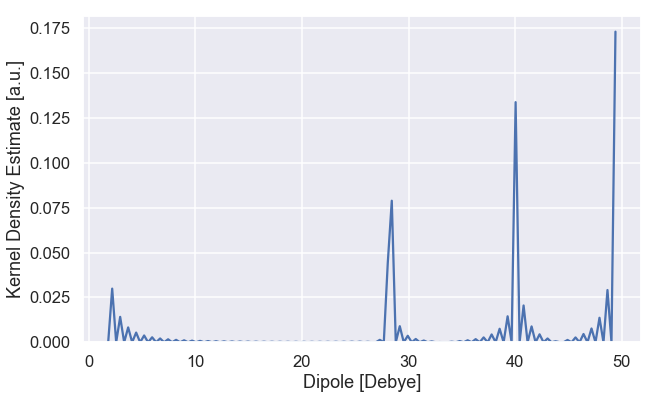
\includegraphics[width=0.9\linewidth]{Figures/System/pc_bad_convergence.png}
            \caption{The Kernel Density Estimate of the total dipole for a sample set of 25 monomer dipole calculations.}
            \label{fig:pc_bad_convergence}
        \end{figure}
        
        Figure \ref{fig:pc_bad_convergence} shows an example of this calculated dipole fluctuations. Here, the same converged wavefunction for a monomer is used to calculate the dipole 25 times, and the kernel density estimate (KDE) for the population is plotted. A peak occurs around the expected value of 1.86 D, but three additional peaks occur for much higher dipole values. (Note, the height of the peak does not necessarily correlate the number of sample with that value and is largely meaningless at this point.) All together, this suggests that some parameter in the system is not well converged.
        
        In an attempt to rectify this issue, a zoo of parameters were put through a tuning process, including: basis set size, $k$ point sampling, box size, number of self-consistent steps, smearing, number of empty bands used in the calculations, and energy difference tolerance. In all cases, similar fluctuations in dipole values resulted. Furthermore, it appears that many people have experienced the exact same issue when attempting to calculated the dipole of a monomer using the VASP and Wannier90 software packages in conjunction with the VASP2WANNIER library [\textbf{mailing list citations}]. 
        
        From reading the identical issues and from personal correspondence with some of the researchers experiencing said issue, the problem likely occurs when the VASP2WANNIER library is called to project the Bloch states on the Wannier states. The only person identified that was able to solve this problem did so by using a different \textit{ab initio} software package [\textbf{cite personal correspondence}]. For sake of consistency and time, however, a different approach is used to overcome this convergence issue.
        
        \paragraph{Removing Outliers} For the MDT case, it is trivial to remove the outliers, because there exists an accepted value in literature. However, for the array of water molecules used to calculate the potential maps, no \textit{a priori} value can be found, necessitating a quantitative and systematic way to determine and remove the outliers. This is accomplished via the modified Z-score.
        
        The modified Z-score is an extension of the standard Z-score 
        \begin{equation}
        \label{eq:z_score}
            Z_i = \frac{x_i - \Tilde{x}}{\sigma},
        \end{equation}
        
        \noindent for measurement $x_i$, sample mean $\Tilde{x}$, and sample standard deviation $\sigma$. Essentially, eq. (\ref{eq:z_score}) transforms the datum $x_i$ into units of standard deviations from the sample mean. Using the Z-score on small sample sizes is known to yield misleading results for small sample sizes [\textbf{citation}].
        
        Rather than use the sample mean, the modified Z-score used the more robust median, since it is less sensitive to large outlier fluctuations. This score is defined as
        
        \begin{equation}
            M_i = \frac{x_i - \Bar{x}}{\mu},
        \end{equation}
        
        \noindent for sample median $\Bar{x}$ and median absolute deviation $\mu$ [\textbf{citation}]. Rejecting the outliers becomes a simple task of tuning a tolerance $s$, for which a modified Z-score that is greater $M_i>s$ identifies an outlier. Note, a smaller $s$ value corresponds to being discriminatory towards outliers.
        
        
        
        \begin{figure}
            \centering
            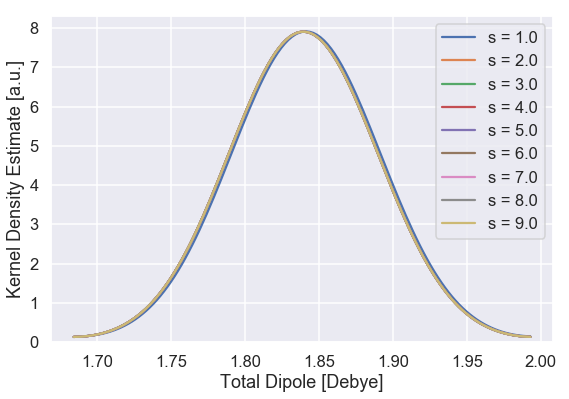
\includegraphics[width=0.3\linewidth]{Figures/System/pc_m_scan_monomer.png}\hfill
            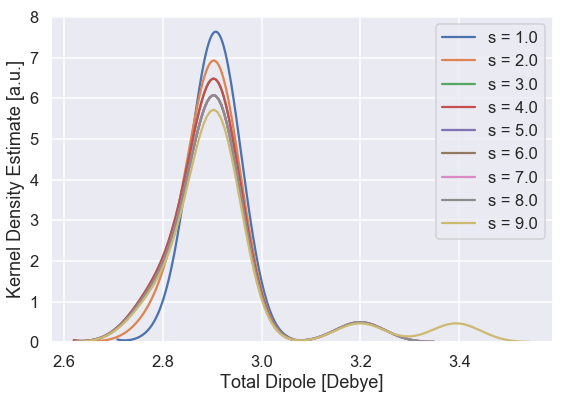
\includegraphics[width=0.3\linewidth]{Figures/System/pc_m_scan_dimer.png}\hfill
            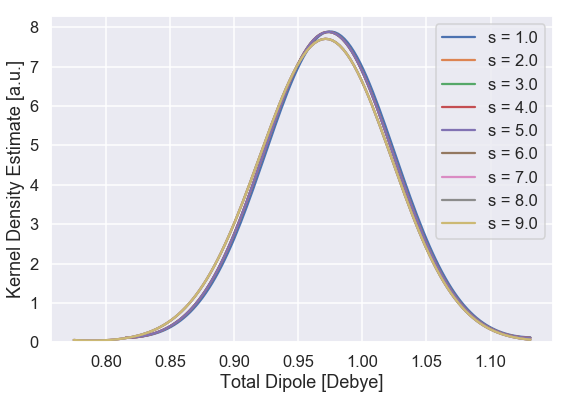
\includegraphics[width=0.3\linewidth]{Figures/System/pc_m_scan_trimer.png}\hfill
            \caption{Tuning results for the modified Z-score tolerance $s$. (Left) Monomer, (center) dimer, (right) trimer.}
            \label{fig:m_scan}
        \end{figure}
        
        Figure \ref{fig:m_scan} shows the monomer, dimer, and trimer total dipole KDEs (left, center, and right therein) for different tolerance values $s$. As seen in all three cases, a well-defined peak is visible. In the case of the monomer and trimer, there appears to be little sensitivity to tolerances over the range investigated. For the dimer, larger dipole peaks appear for the larger tolerance (less discriminatory) values. These vanish for $s<6$, and the peak is maximized for $s=1$. Therefore, for sake of consistency, $s=1$ is used for all outlier rejections throughout.
        
        One more note on the outlier removal procedure. Generally, there are two different data sets of dipole values on which one could detect outliers---the individual dipoles and the total system dipole. In order to maximize the signal-to-noise ratio, the modified Z-score should be calculated on the total dipole, and if it is determined to be an outlier, \textit{all} of the individual dipoles that correspond to that total dipole value should be discarded. The underlying assumption being that if the total dipole is an outlier, then the calculation was not well-converged and the individual dipole measurements are not reliable.
        
        \begin{figure}
            \centering
            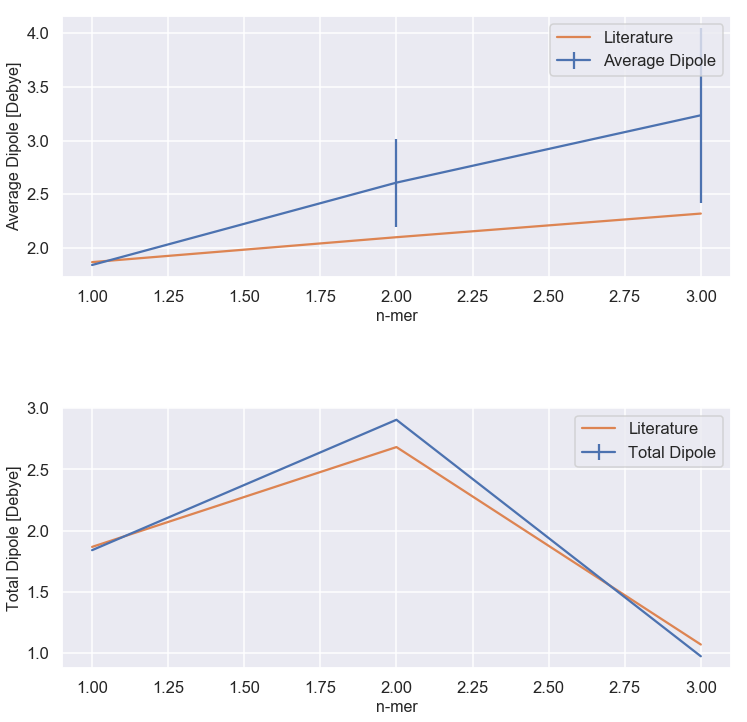
\includegraphics[width=0.9\linewidth]{Figures/System/pc_benchmark_results.png}
            \caption{Results for the n-mer partial charge benchmark. (Top) Average individual dipole; (bottom) total system dipole.}
            \label{fig:pc_bench_results}
        \end{figure}
        
        \subsection{Results and Analysis} The results for the n-mer partial charge benchmark using the above described Wannierization, charge assignment, and outlier removal are compared to literature results [\textbf{n-mer citation}] in Fig. \ref{fig:pc_bench_results}. Here, error bars represent the standard error of the mean and are not visible within the resolution of the bottom graph. Clearly, the results are in good qualitative and quantitative agreement with the literature values. Discrepancies between the two are attributed to the use of differently optimized structures, different basis sets, and different functionals. 
        
        As such, the above described procedures are deemed appropriate to use in order to perform partial charge analysis on the beryl and vacuum systems.
        
    \section{Extra-Framework Water Analysis}
    
    Having established the efficacy of the proposed partial charge analysis method, the average dipole as a function of fill, rotation, and local environment are investigated. However, a resource-imposed limitation is highlighted.
    
    The cost for collecting a large enough sample size to perform any meaningful dipole of statistical analysis on the water molecule dipoles is quite high. In the case of the benchmark, 25 runs for each system were calculated, with a nearly 50\% rejection rate. For the actual system under investigation, there exists 60 different configurations for each fill type, and each one of those requires multiple runs. For the vacuum case, it is feasible to do the same number of runs (i.e. 25) as the benchmark, with run times of about 12-14 days. For the beryl case, there exist nearly 20 times as many ions and electrons, and only 5 runs per configuration can be run in the same amount of time. 
    
    Therefore, vacuum case results are prioritized, for both the vacuum-geometry and beryl-geometry water molecules. This allows for an attempt at parameterization to establish proof-of-concept (see Appendix \textbf{parameter test section}, without having to run all of the expensive beryl-case calculations (not to mention trying to fit the dipole-framework interaction to an acceptable analytic function). Even still, data for the beryl cases will be collected up until point of submission, and the results attained will also be reported below.
    
        \subsection{Vacuum Case}
        \label{sec:pc_vacuum_Case}
        
        \textbf{Procedure} As mentioned above, the relatively small system size for the vacuum case allows for a larger sample size to be collected. Specifically, for both the vacuum-geometry and beryl-geometry water molecules, the individual and total dipoles are calculated according to the benchmark procedure 25 times for each self-consistent configuration calculated during the potential map investigation. Outliers rejection tolerance is set to $s=1$.
        
        \textbf{Results and Analysis} Figure \ref{fig:pc_vacuum_kde} gives the KDEs for the individual dipoles for both the vacuum- and beryl-geometry water molecules (left and right, respectively therein) as a function of fill and for all configurations. For the vacuum-geometry case, the results for fill 1000 are omitted for ease of reading, but an almost $\delta$-function-like peak occurs for $p = 1.96$ D. While a quantitative comparison is not discernible from this figure, it is clear that describing the dipole data sets in an average manner is appropriate.
        
        \begin{figure}
            \centering
            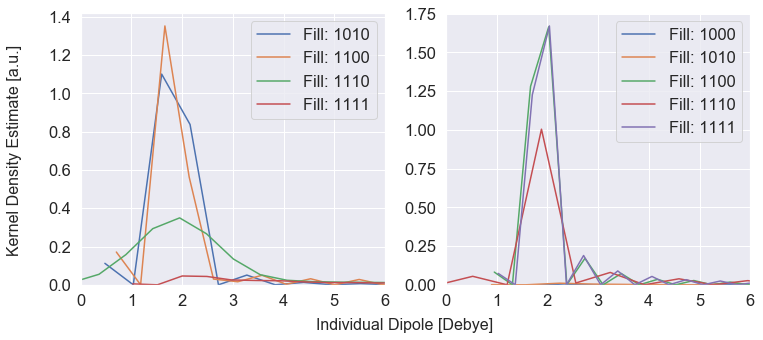
\includegraphics[width=0.9\linewidth]{Figures/System/pc_vacuum_compare_kde.png}
            \caption{The individual dipole KDEs by fill for the vacuum- (left) and beryl-geometry (right) water molecules in vacuum. Note, for the vacuum-geometry case, the results for the 1000 fill case are omitted for clarity.}
            \label{fig:pc_vacuum_kde}
        \end{figure}
            
        The average individual dipole as function of fill for water molecules with both the vacuum-geometry (solid, blue line) and beryl-geometry (dashed, black line). In general, the qualitative behavior of the dipole as a function of fill does not change drastically with respect to geometry, which is as expected. The main difference appears to be a contraction effect of the dipole when moving from the vacuum- to beryl-geometry water molecules. These results are consistent with the structural optimization results found in Section \ref{sec:geom_opt}. Namely, the framework has a dilating effect on the water geometry, with both the blond length $r$ and OHO angle $\theta$ increasing (the latter being more significantly increased than the former). 
        
        If the water molecule is thought of being positioned as in Fig. \ref{fig:pc_analysis}, the individual dipole is along the $+x$-direction, and the magnitude $p$ is proportion to the projection of $r$ on the $x$-axis. That is, 
        
        \begin{equation}
            p \propto r \cos\left(\frac{\theta}{2}\right).
        \end{equation}
        
        \noindent Since the percent difference between the 25\% and 100\% fill is greatest for the OHO angle $\theta$ (approximately 1.1\5 compared to 0.1\% for the bond length $r$), the bond length can be thought of to be nearly constant. Therefore, as the angle $theta$ increases, the projection onto the axis decreases---and so goes the dipole magnitude.
        
        \begin{figure}
            \centering
            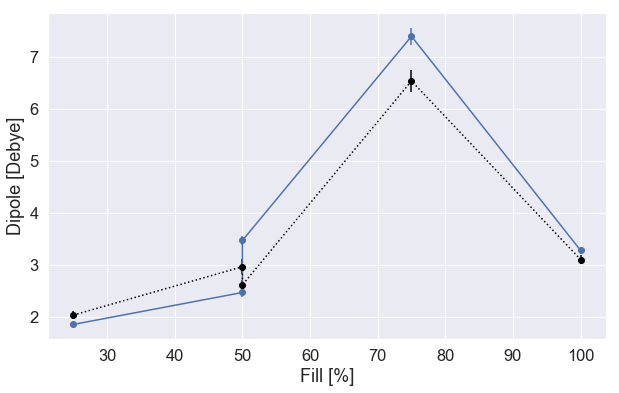
\includegraphics[width=0.9\linewidth]{Figures/System/pc_vacuum_avg_dipole.png}
            \caption{The average individual water molecule dipole as a function of fill. Again, the solid, colored line represents vacuum-geometry results, while the dashed, black line represents beryl-geometry results. Error bars represent the standard error of the mean.}
            \label{fig:pc_vacuum_avg_dipole}
        \end{figure}
        
        The contraction-inducing influence on the dipole moment does not universally result in an increase or decrease in dipole moment, as shown in Fig. \ref{fig:pc_vacuum_dipole_ratios}. Here, the average individual dipole moment ratio between the vacuum- and beryl-geometry water molecules is given as a function of fill. The red line indicates unity, and therefore, ratios below (above) unity indicate a(n) decrease (increase) in the dipole moment when moving from the vacuum- to beryl-geometry. A decrease is observed for fill 25\%, and an increase is observed for the remaining fills. 
        
        \begin{figure}
            \centering
            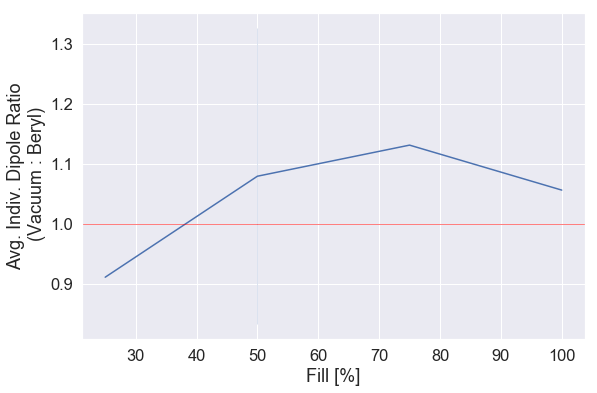
\includegraphics[width=0.9\linewidth]{Figures/System/pc_vacuum_dipole_ratios.png}
            \caption{The ratio of the individual dipole (vacuum- to beryl-geometry} as a function of fill. The red line denotes unity.
            \label{fig:pc_vacuum_dipole_ratios}
        \end{figure}
        
            \subsection{Partial Charge Assignment}
            \label{sec:pc_assign}
            
            Using the dipole results in conjunction with the structural optimization results, the partial charges are assigned using the following procedure.
            
            \begin{figure}
                \centering
                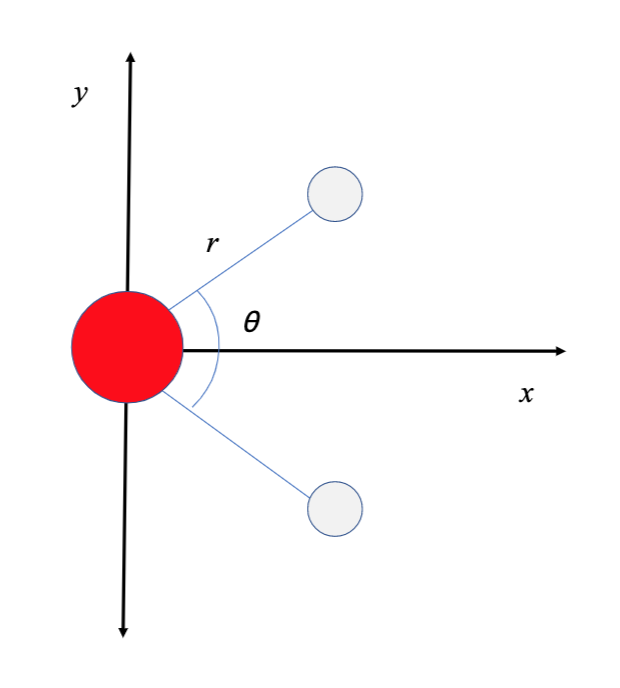
\includegraphics[width=0.5\linewidth]{Figures/System/pc_analysis.png}
                \caption{Diagram of a model molecule in the $xy$-plane with the oxygen atom centered at the origin. See text for details.}
                \label{fig:pc_analysis}
            \end{figure}
            
            \paragraph{Procedure} Consider first a water molecule in the $xy$-plane, with the oxygen atom at the origin and hydrogen atoms at $(r\cos\alpha,\pm r\sin\alpha)$ with $\alpha - \theta/2$, as shown in Fig. \ref{fig:pc_analysis}. The dipole magnitude is given by
            
            \begin{equation}
            \label{eq:dip_mag}
                p = 2n_H|e| r \cos\left(\frac{\theta}{2} \right)\hat{x},
            \end{equation}

        \noindent for hydrogen atom partial charge assignment $n_H > 0$ and elementary charge $e$. From (\ref{eq:dip_mag}), the partial charge assignment for the oxygen and hydrogen atoms are given, respectively, as
        
        \begin{eqnarray}
        \label{eq:pc_assign}
            n_H &=& \frac{p}{2er} \sec\left( \frac{\theta}{2} \right)  \\
            n_O &=& -2n_H 
        \end{eqnarray}
        
        \paragraph{Results and Analysis} The partial charge assignment for the oxygen atom is given as a function of fill in Fig. \ref{fig:pc_vacuum_pc}. In qualitative terms, the results are equivalent to the dipole results in Fig. \ref{fig:pc_vacuum_avg_dipole}, although here in the negative since oxygen is electronegative. A distinct feature is apparent for the 100\% fill case, however, in that the partial charge assignment appears to be close to identical. In fact, systematically the difference between the geometry cases appears to be indirectly proportional to fill, with the except of the degenerate 50\% cases, wherein the partial charge also appears to be nearly identical.
        
        \begin{figure}
            \centering
            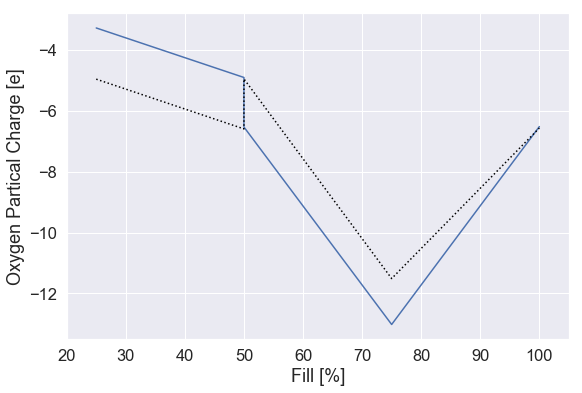
\includegraphics[width=0.9\linewidth]{Figures/System/pc_vacuum_pc.png}
            \caption{The oxygen partial charge assignment as a function of fill for the vacuum- (solid,blue line) and beryl-geometry (dotted, black line) water molecules.}
            \label{fig:pc_vacuum_pc}
        \end{figure}
        
        These observations are explored deeper with the help of Fig. \ref{fig:pc_vacuum_pc_ratios}. Here, the ratios of the vacuum- to beryl-geometry oxygen partial charge assignment are given as a function of fill. The red line indicated unity. Again, the qualitative behavior here is similar to that in Fig. \ref{fig:pc_vacuum_dipole_ratios}, and the fill 50\% and fill 100\% cases are closest to unity. The minimally filled case represents the greatest discrepancy between the two geometry cases.
        
        \begin{figure}
            \centering
            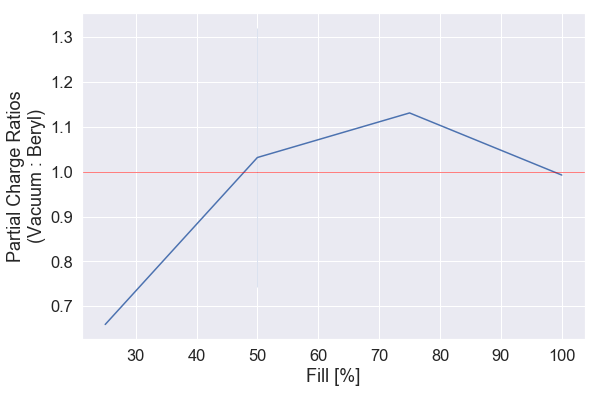
\includegraphics[width=0.9\linewidth]{Figures/System/pc_vacuum_pc_ratios.png}
            \caption{Oxygen partial charges ratios between the vacuum- and beryl-geometry cases as a function of fill. The red line indicated unity.}
            \label{fig:pc_vacuum_pc_ratios}
        \end{figure}
        
        
        \subsection{Beryl Case}
        \label{sec:pc_beryl_case}
        
        As mentioned before, determining the Wannier centers, and hence the partial charge, for the water molecules in the beryl framework is quite expensive. In the same amount of time that the vacuum case calculations can be made 25 times per configuration, only ten in-framework calculations per configuration can be performed. Due to time limitations, it is unclear if all of the fills will be investigated before completion of this work, but what results are attained are reported below.
        
        \paragraph{Procedure} The same procedures as utilized in the vacuum cases are used for both the generation of the Wannier data and the partial charge assignment. As noted, however, only ten Wannier calculations are performed for each configuration.
        
        \paragraph{Results and Analysis} The preliminary results for the average individual dipole for water molecules in the beryl framework (red) are given in Fig. \ref{fig:pc_beryl_pc}. For comparison, the results for vacuum cases with beryl- and vacuum-geometry (blue and green, respectively) are provided for comparison. As expected, the smaller sample size manifests itself as a greater error in the average dipole compared to the vacuum cases. Furthermore, the average dipole for the beryl-geometry in vacuum case and in-beryl case are indistinguishable from each other when considering the error. Whether or not they would remain distinguishable as better statistics are achieved is uncertain, but the prospect hints at a more efficient way of calculating the dipoles. Namely, use the in-framework geometry in the vacuum case---saving potentially weeks of calculations. Also, if this indistinguishability holds, it would support the idea that the framework interacts nominally with the dipole-dipole system.
        
        \begin{figure}
            \centering
            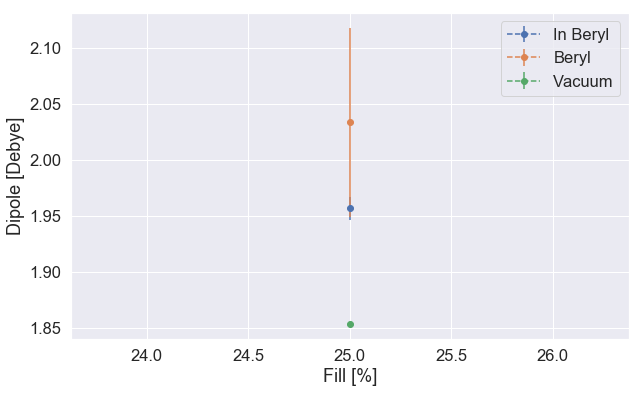
\includegraphics[width=0.9\linewidth]{Figures/System/pc_beryl_pc.png}
            \caption{The average individual dipole moment as a function of fill for extra-framework water molecules in the beryl framework (red). The vacuum cases with vacuum- and beryl-geometry (green and blue, respectively) are provided for comparison.}
            \label{fig:pc_beryl_pc}
        \end{figure}
        
        The discrepancy between partial charge is even less than that for the dipole, with the in-framework and beryl-geometry vacuum cases agreeing to six decimal places (a few orders of magnitude greater accuracy than this study is claiming) for the oxygen atom partial charge
        
        \begin{equation}
            q_O = -4.947902\text{ } |e|.
        \end{equation}
        
    \section{Summary and Outlook}
    
    Overall, the partial charge analysis stage proves to be the biggest bottleneck in terms of computational resources needed. As discussed in Section \ref{sec:benchmark}, this is because of a known convergence issues in the Wannierization procedure using VASP, Wannier90, and the VASP2WANNIER library. Even still, a workable procedure that involves rejecting outliers using the modified Z-score is identified and used to benchmark the cases of the water monomer, dimer, and trimer (Section \ref{sec:convergence_issue}). The results for both individual dipole and total dipole generally agree with the results found in literature, providing confidence in the prescribed procedure.
    
    Overcoming this convergence issue should be a primary focus for future studies, and said studies would be advised to use the water n-mer cases as a benchmark when choosing functionals, basis sets, etc. Also, over partial charge analysis methods (e.g. DDEC6) may yield better results under different approximations. If such a set of approximations can be found, using DDEC6, for example, would results in orders of magnitude decrease in the cost of this step.
    
    Next, the vacuum case for extra-framework water molecules---both with vacuum- and beryl-geometry---is examined in Section \ref{sec:pc_vacuum_Case}. Both geometry cases exhibit similar dipole as function of fill behavior, but the beryl-geometry case experiences a \textit{contraction}-like effect that is consistent with the \textit{dilation}-like effect on geometry found previously. As mentioned numerous times before, examining larger sample sizes with greater fill degeneracy would be of particular interest, because it would allow for a more general dipole versus fill curve to be found.
    
    A procedure for using the optimized geometry results and dipole results to determine the partial charge assignments in outlined in Section \ref{sec:pc_assign}. The resulting oxygen partial charge assignments mirror the dipole results in the sense that the differences between the two geometry cases are qualitatively negligible. For the partial charge; however, there is less discrepancy in partial charge assignment between the two geometry types than the dipole magnitudes.
    
    Finally, preliminary results for the case of extra-framework water molecules in the beryl crystal are provided in Section \ref{sec:pc_beryl_case}. As discussed, these calculations are significantly more expensive than the vacuum counterparts, and only a partial data set is available as of time of writing. From the available results, it appears that very little difference in dipole magnitude, and even less difference in partial charge assignment, exists between the beryl-geometry in vacuum and the in-beryl cases. If this trend holds as more data is attained, it would suggest a significant increase in productivity by allowing for partial charge assignment as calculated in vacuum. Having the dipole-framework contribution parameters as degrees-of-freedom also makes this approach more plausible.